\documentclass[12pt]{article}
\usepackage{amsmath}
\usepackage{authblk}
\usepackage[utf8]{inputenc}
\usepackage{subcaption}
\usepackage{natbib}
\usepackage{graphicx}
\usepackage{float}
\restylefloat{table}
\usepackage{array}
\usepackage[hidelinks]{hyperref}
\usepackage[table]{xcolor}%http://ctan.org/pkg/xcolor
\setlength{\parindent}{0pt}


\usepackage[a4paper,width=165mm,top=25mm,bottom=25mm]{geometry}
\graphicspath{ {./Pictures/} }
\title{\Huge Project Plan}
\author{Axel Trolme \& Martin Friberg}

\begin{document}
\maketitle
\vfill

\includegraphics[width=\linewidth]{Pictures/logo_heartbyte_transparent_v_1_1 (1)}

\vfill
\begin{center}
        \textbf{\large Current Version 5.0 [2020-12-08]}
\end{center}
\clearpage

\section{Change Log}
	
\begin{table}[H]

\begin{center}
\begin{tabular}{ | m{2cm} |m{2cm} |m{5cm}|m{4cm}|m{3cm}| } 
\hline
{Version Number} & {Published Date} & {Description of Revision}& {Author}& {Approved By} \\ 
\hline
1.0 & 2020-10-02 & First version of the project plan & Martin Friberg & Partik Palmgren \\
\hline
1.1 & 2020-10-14 & Added tollgates and goals for the project as a table, time and resource plan enhanced & Axel Trolme & Partik Palmgren \\
\hline
2.0 & 2020-11-15 & Enhanced description of the organization roles, Stronger words in explanation of risks, enhanced tollgate description and Gantt-chart for development & Axel Trolme & Partik Palmgren\\ 
\hline
3.0 & 2020-11-24 & Enhanced description of iterations, risk actions improved, table of contents added, overall language changed, change order of information & Axel Trolme & Emma Johansson \\ 
\hline
4.0 & 2020-12-06 & Enhanced language \& overall minor corrections& Axel Trolme & Patrik Palmgren \\ 
\hline
5.0 & 2020-12-08 & Added links to GitLab for all the documents mentioned in the text & Axel Trolme & Patrik Palmgren \\ 
\hline
\end{tabular}
\end{center}
\caption{\label{tab:changeLog}Document change log}
\end{table}
\clearpage
\tableofcontents
\clearpage

% Introduction
    \section{Project background}
    \setlength{\parindent}{0pt}
The text below describes the background to the project HeartByte is currently working on, to develop a self-care system for Region Östergötland.

\subsection{Customer introduction \& main focus}
HeartByte has got a new project with the customer Region Östergötland, a region within the Swedish healthcare system who sees a possibility in extending the self-care treatment for a chosen group of patients with chronic diseases. With this system, Region Östergötland believe they can reduce the occupancy rate at the hospitals as an effect of patients not having to visit the hospital recurrently. \vspace{5mm}

Region Östergötland says these patients can be monitored by letting them selves do their samplings of tests at home, and given care through a web based system that HeartByte is to deliver. In order to create customer value, Region Östergötland needs a system to handle and monitor many patients at once with focus on good usability for the employees and care givers.

\subsection{Relevant constraints}
The product delivered to Region Östergötland is be delivered for free. Due to this, HeartByte does not have an ordinary budget to keep track off with cash equivalents. Instead, HeartByte has a budget made up of hours that has to be taken in consideration. \vspace{5mm}

HeartByte has put together a group of 26 employees with complementary skills with 160 hours each to spend throughout the entire project. This leaves the budget at $26 \cdot 160 = 4160$ hours. Furthermore, there is a list of general constraints for the final product to meet:

\begin{itemize}
    \item The system has to be available for fixed Windows workstations.
    \item The system has to be available for tablets. 
    \item It has to be a customizeable dashboard available, meaning that the care giver to a limited extent should be able to decide what information and modules that is to be presented for the user.  
    \item When accessing data from the patient records, Open EHR APIs has to be used
    \item When accessing data from the patient records, the action has to be logged in the system for an admin user to retrieve if needed.
\end{itemize}

A detailed list of functional and non-functional requirements applicable to the product is to be found in the project's SRS-document.

\subsection{Project goal}
The goal of the project is to deliver a product satisfying the requirements given by the customer. In order to assure the final product meeting the customers quality demands, sub-goals for the project has been set. See the table below for more information.

\begin{table}[]
\begin{tabular}{|l|l|}
\hline
\multicolumn{1}{|c|}{\textbf{Goal}}& \multicolumn{1}{c|}{\textbf{Meaning}}\\ \hline
Implement continuous delivery & Make possible to external stakeholders to monitor the progress \\ \hline
\begin{tabular}[c]{@{}l@{}}Use a CI-environment for the used \\ repository\end{tabular} &\begin{tabular}[c]{@{}l@{}}Mitigate and avoid major 
issues when pushing new code to\\ the repository by running unit tests for intended functionality\end{tabular}\\ \hline
Document all processes & \begin{tabular}[c]{@{}l@{}}To create a reliable \& effective structure of the project,\\ its processes should be documented and updated\end{tabular}\\ \hline
Deliver weekly status reports & \begin{tabular}[c]{@{}l@{}}To keep the entire organization and external stakeholders\\ updated regarding current tasks and progression\end{tabular}\\ \hline
Use a bug-tracking system& \begin{tabular}[c]{@{}l@{}}To make the process of debugging easier. Git issues is \\ to be used\end{tabular}\\ \hline
\begin{tabular}[c]{@{}l@{}}Use a traceability system for \\ tasks and requirements\end{tabular} & \begin{tabular}[c]{@{}l@{}}To increase the satisfaction of the customer, a traceability-\\ system between features, tasks and requirements is to be \\ used. GitLab is to fulfill this task.\end{tabular} \\ \hline
\begin{tabular}[c]{@{}l@{}}Internal followup on relevant \\ documents\end{tabular} & \begin{tabular}[c]{@{}l@{}}In order to increase the value of having living documents, \\ they also have to be updated accordingly as the project \\ makes progress.\end{tabular} \\ \hline
\end{tabular}
\caption{\label{tab:table-name}Internal project goals.}
\end{table}
\subsection{Start and expected end date}
\begin{itemize}
    \item The start of this project is 2020-09-09
    \item Intended and planned code stop set to 2020-12-04
    \item The delivery of final end-product at VSSE 2020-12-10
\end{itemize}
    \clearpage
% Theory
    \section{Time and resource plan}
    
\subsection{Time and resource plan}
\subsection{Milestones}
\subsection{Tollgates}
\subsection{Deliverables}
\subsection{Activities}
\subsection{Resources}

\clearpage
% Methods
    \section{Project organization}
    This chapter covers the basic setup of the organization, how work is done in the project as well as ways of communication. 

\subsection{Roles}
Members of the organisation applies for different positions within the organisation. figure \ref{fig:company structure} shows the outcome of the application process. The organisation is divided into two different departments, 'Research \& Development' and 'Product \& Sales' department. A board of external stakeholders supporting the organisation is also constructed.  

\begin{figure}[hbt!]
\centering
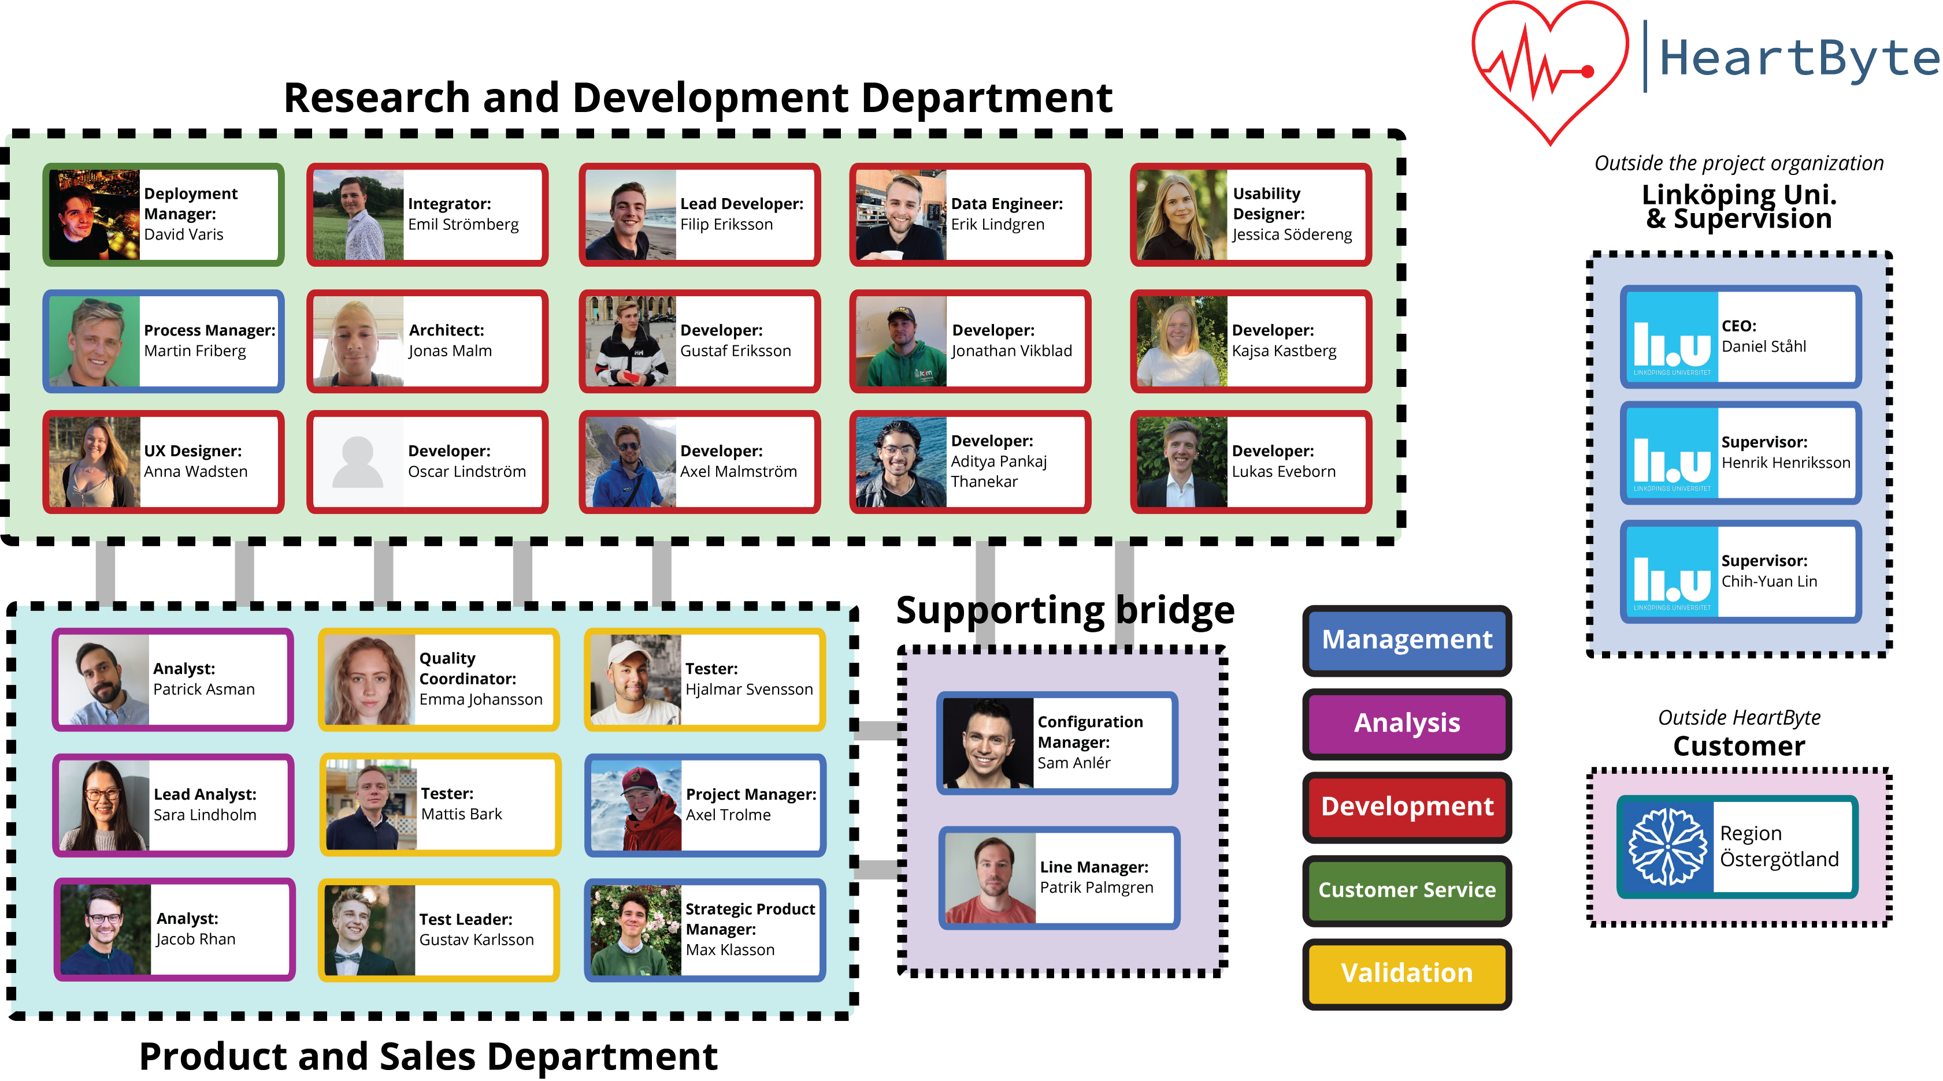
\includegraphics[width=\linewidth]{Pictures/Organization.png}
\caption{HeartByte project group}
\label{fig:company structure}
\end{figure}

Within and across the aforementioned departments are also a number of smaller groups. These groups are responsible for working with a certain task such as testing, developing, analyzing the system or managing the groups. Cross-functional teams are created in order to apply a broader knowledge when developing a certain feature or working with a certain task requiring knowledge from different departments. For example, analysts are included when developing a feature in order to assure that the quality and function of the feature is in line with what the software is supposed to achieve according the the applicable requirements. \\ 

The different roles within the organization all fills different purposes. The main goal is to create an organization able to deliver the product ordered by the customer, on time and with intended quality. For this purpose, the organization is built up by different teams, see description below. 
\begin{table}[H]

\begin{center}
\begin{huge}
    Management
\end{huge}
\begin{tabular}{ | m{4cm} |m{3cm} |m{10cm}| } 
\hline
\textbf{Position} & \textbf{People} & \textbf{Description} \\ 
\hline
Project Manager & Axel Trolme & Ensures that the goals for the project are met by planning and following up the tasks, as well as planning the resource allocation. Also responsible for communication with the company CEO Daniel Ståhl. \\
\hline
Process Manager & Martin Friberg & Decides and structures the processes that are to be used throughout the project. Communicates with the different departments of the project organisation in order to map what education plans they need in order to fulfill given tasks.  \\
\hline
Strategic Product Manager & Max Klasson & Responsible for communication with the customer as well as with the analysis team. They also decides how the product features should be prioritized and has to keep a constant communication with the different departments and groups within the project.  \\
\hline
Configuration Manager & Sam Anlér & Responsible for deciding what artefacts and documents that are to be put under version control and what parts of the product that should be available for a specific release. Also, Sam has become responsible for pursuing company health evaluations every second week. They also ensures that the resources given to the project in terms of tools are used properly and therefore has a constant communication with the development team. \\
\hline
Line Manager & Patrik Palmgren & Responsible for book keeping and the structure of the documents, to make sure that they are stored in the correct way and that the documents are updated accordingly when needed. Also, Patrik is responsible for communicating with the different groups within the company in order to get a clear picture of what's needed to put in the different documents.   \\
\hline
\end{tabular}
\end{center}
\caption{\label{tab:table-name}Description of project roles within management}
\end{table}
\vspace{10cm}
\begin{table}[H]

\begin{center}
\begin{huge}
    Development
\end{huge}
\begin{tabular}{ | m{4cm} |m{3cm} |m{10cm}| } 
\hline
\textbf{Position} & \textbf{People} & \textbf{Description} \\ 
\hline
UX Designer & Anna Wadsten & Expert on how the interaction between the user and the product / system is to be performed. Anna has also been our chief in command for the development of the Hi-Fi as well as Lo-Fi prototypes, and has a constant contact witht the customer in order to brief the design of the prototypes with the end users. The UX designer has also been involved in the process of user testing in order to be able to bring the information from these tests into the development of the prototypes.  \\
\hline
Architect & Jonas Malm & Is responsible for what target environment to be in use when developing the product. They is also the responsible person for making key decisions regarding the hgh-level architecture. Also, Jonas makes sure that our non-functional requirements are met as well as judging future capabilities and outcomes of design decision being made.  \\
\hline
Integrator & Emil Strömberg & Responsible for putting the different pieces of software developed together, in order to create a functional product.  \\
\hline
Lead Developer & Filip Eriksson & Leads the work for the developers and hands out the tasks to the different groups within the development team. Also, Filip is the SCRUM-master on the weekly SCRUM-meetings being held for the development group. This way of working enhances the productivity and flow of information through the team. \\
\hline
Usability Designer & Jessica Södereng & Works in close connection with Anna Wadsten with development of the Hi-Fi and Lo-Fi prototypes. Also, Jessica is responsible for designing the navigation through the system that the end-user will work with. \\
\hline
Data Engineer & Erik Lindgren & Prepares the infrastructure and integrates the data from different sources. Since the product developed isn't much about big data, Eriks position within the company has became an ordinary developer working alongside Filip Eriksson as lead developer as well as the other developers. \\
\hline
Developer & Oscar Lindström, 
Gustaf Eriksson, 
Axel Malmström, Jonathan Vikblad, Aditya Pankaj Thanekar, Kajsa Kastberg, Lukas Eveborn   & Writes the code and develops the software components that the system / product is be built up from. Reports to Filip Eriksson (Lead Developer). \\
\hline
\end{tabular}

\end{center}
\caption{\label{tab:table-name}Description of project roles within development}

\end{table}
\begin{table}[H]

\begin{center}
\begin{huge}
    Customer Service
\end{huge}
\begin{tabular}{ | m{4cm} |m{3cm} |m{10cm}|| } 
\hline
\textbf{Position} & \textbf{People} & \textbf{Description} \\ 
\hline
Deployment Manager & David Varis & Responsible for making the product available for the customer, including launching the product with docker as well as making it available as a web application. \\
\hline
\end{tabular}


\end{center}
\caption{\label{tab:table-name}Description of project roles within Customer Service}

\end{table}
\begin{table}[!hbtp]

\begin{center}
\begin{huge}
    Validation
\end{huge}
\begin{tabular}{ | m{4cm} |m{3cm} |m{10cm}| } 
\hline
\textbf{Position} & \textbf{People} & \textbf{Description} \\ 
\hline
Quality Coordinator & Emma Johansson & Responsible for measuring the product in terms of requirement-specific metrics as well as initation of needed changes and fixes. Emma determines the quality of the product, and organizes the reviews of both software and documents.  \\
\hline
Test Leader & Gustav Karlsson & Works in close connection with both the development team and the analysis team. The main responsibilities for the test leader is to evaluate our requirements and to make sure that test are developed in order to realize the testing of the product. Also, Gustav is responsible for organizing the process reagrding user tests.   \\
\hline
Tester & Hjalmar Svensson \& Mattis Bark & Works in close contact to the test leades, Gustav Karlsson, and assists him in the development of the tests needed. Both automated tests as well as user tests are developed by the testers \\
\hline
\end{tabular}


\end{center}
\caption{\label{tab:table-name}Description of project roles within Validation}

\end{table}
\begin{table}[!hbtp]

\begin{center}
\begin{huge}
    Analysis
\end{huge}
\begin{tabular}{ | m{4cm} |m{3cm} |m{10cm}| } 
\hline
\textbf{Position} & \textbf{People} & \textbf{Description} \\ 
\hline
Lead Analyst & Sara Lindholm & Responsible for defining and describing the requirements that the system are to meet. Sara is responsible for keeping up the communication with the customer regarding the requirements, and to documents these decisions in the SRS-document.  \\
\hline
Analyst & Jacob Rahn \& Patrick Asman & Assists the lead analyst, Sara Lindholm, in the communication with the customer as well as in the process of defining and describing the requirements. \\
\hline
\end{tabular}


\end{center}
\caption{\label{tab:table-name}Description of project roles within Analysis}

\end{table}

\subsection{Knowledge \& skill}
The company management sends out a form to the organisation where the members fill in what knowledge they have from before and what knowledge they are currently lacking. In this way, management is able to locate in what areas the skill and knowledge is high and what areas are lacking skill and knowledge. The languages chosen by the architect, Jonas Malm, for developing our Handle Many Platform is as mentioned React for front-end development and a combination of Flask and Python for the back-end development. According to the skill survey, the knowledge and skill within React is fairly limited. This fact has made the management produce a short term plan for introducing the new environment to the developers, where the first step is to watch the tutorial videos regarding React. In regards to further development the management outsources the major responsibility of sharing knowledge, acquiring a knowledge base and making the development of the project to the lead developer Filip Eriksson. For more information, see the \href{https://gitlab.liu.se/tddc88-company-3-2020/deploy/-/tree/Document_branch/Education_plan}{\underline{education plan}}. 

\subsection{Training}
When working on the project, new skills has to be developed among the team members. For this purpose, different ways of training and education is provided. The sections below give a brief description of how this is achieved. For more detailed information, see the \href{https://gitlab.liu.se/tddc88-company-3-2020/deploy/-/tree/Document_branch/Education_plan}{\underline{education plan}} document. 
\subsubsection{Workshops}
When development methods include new tools, an organisation member responsible for the area is chosen. This person is supposed to gain a deeper understanding about the aforementioned tool. The person mentioned is then in charge of making sure that the rest of the team that is supposed to work with the tool gains the required knowledge about it. This is done via workshops online where the responsible person goes through the basics of the tool.  A workshop could also include different brainstorming activities, where the participants are to come up with ideas regarding risks, company name, requirements for the system or tools to use for a specific system. 

\subsubsection{Presentations}
The management produces presentations to hold during CEO meetings to educate the team in what has been done during the week and what is to be done during the upcoming weeks. The management is also highlighting the tasks most critical to get done as soon as possible. The presentations is also used to educate the team in processes and tools that makes the work more effective. Example of tools included is GitLab, Microsoft Teams and different programming languages. The presentations can also focus more on education, for example how to handle documents and where to place them to be easily found once they are needed. The focus is to provide the team with the skills and information needed. To find more information regarding education, please see the education plan document. 

\subsubsection{Resource sharing}
Through sharing resources in Teams and GitLab the team spreads the knowledge and progression within their work. This enables the whole team to take part of each others knowledge and where they currently are in terms of progression. It also prevents two people from doing the same thing on two different ends. 

\subsection{Communication and reports}
Since the organization is fairly big with 26 members,  structured ways in how communication throughout the team is handled, is highly needed. The sections below gives insight in this process. 
\subsubsection{Group meetings and Discussions}
As stated above, the organisation is separated into two departments. From these departments, cross-functional teams and teams where the whole group is working together on a specific task is created. The cross-functional teams makes it easier to share the information between the research and development department and the product and sales department as well as between the different specialized groups of analysts, testers, developers and management. Project group meetings takes place at least once every week where the CEO of the company as well as the entire project group is present. Alongside with these meetings other cross-functional meetings are to take place where the groups gets feedback from supervisors of the project. From the supervisors, the cross-functional teams can discuss problems, ideas and functionality of the software or other project related topics. 

\subsubsection{Communication directives}
The task specific groups reports to the team leader of their group. Matters of importance are then to be communicated between different team leaders and management in order to lower the amount of group members that have to have direct communication with each other. This way of communicating also helps the project group and in particular the management to assure that information that concerns parts of, or the entire project group, reaches the members concerned. Team leaders may also have direct contact with each other regarding a task that is specific to only their teams. When the cross-functional teams are set up for a specific task, the team members of the task is of course meant to have direct contact with each other, but if important matters arise, they are to be communicated to their team leaders who can forward the information to management. Management is then to produce a plan to circumvent or deal with the situation. 

\subsubsection{Reports}
In order to keep the stakeholders satisfied and up to date with what is going on in the project, the team announces weekly status reports. The status reports contains information regarding what the group has done during the last week, what is most crucial to be done during the upcoming week as well as a time report. This can also help the CEO keep track of the time spent in the project in order to not exceed the budget. There are also certain living documents that are to be produced in order for the entire team to stay updated about what the latest specifications are for the project. An updated version of the living documents are to be put in the general folder in the shared Microsoft Teams channel at the start of iterations 2-4. The updated documents are to be inspected by document responsible manager Patrik Palmgren in order to assure quality of the documents. 

\clearpage
% Resultat
    \section{Risk management}
    When working with a project, a key aspect is to define risks and to map out in what areas they might appear. This makes it easier to be prepared and to handle the risks once they appear. 
\subsection{Risks, probability, impact and the mitigation and contingency plans}
In order to develop and create a successful project, it is crucial to acknowledge the risks that are present that is hard to avoid completely. The team leaders of the project group talked with their team members and had a discussion regarding what risks that they believed could arise that is hard to avoid completely. The risks that was brought to the table can be seen in the table below. 

\begin{table}[h!]

\begin{center}
\tiny
\begin{tabular}{ | m{0.3cm} |m{2.8cm} |m{0.65cm} |m{0.6cm} |m{0.6cm} |m{0.6cm} |m{0.7cm} |m{0.6cm} |m{2.8cm} |m{2.8cm} | } 
\hline

risk nr & Description & Proba bility & Impact&Risk magnitude  & Project Specific Y/N & Direct/ Indirect & Avoid/ Transfer/ Mitigate & Explanation & Mitigation \\ 
\hline
1 & Git version handling & 3 & 3 & \cellcolor{yellow!40}9 & Y & Direct & Mitigate & Someone in the project overwrites an old 
working feature of the master branch without them knowing & We appoint someone responsible to handle tests for the master branch 
and makes sure that the master branch is working at all times. \\ 
\hline
2 & Our development environment for the CI stops working in GitLab & 1 & 3 & \cellcolor{green!40}3& N & indirect & mitigate & If the environment for the CI stops working the code can not be validated and tested through the CI. Since CI is a vital part of keeping a good standard of code and to minimize the risk of bugs in the deployment this is a risk for the project & In order to mitigate the risk we can use an external git handler that has a functioning CI and use this to test the code where after the code is pushed to our repository \\ 

\hline

3 & We do not get the possibility of doing user tests with the end user & 2 & 4 & \cellcolor{yellow!40}8& N & indirect & mitigate & The lack of user tests with the end user makes us create functionality that they can not use and makes us miss implementing crucial software functionality & The risk can be mitigated by making user tests with the end user continuously, since we might not get the chance of doing so in the end of the project. We might also have to do user tests with users that are not the end users and can from that find "obvious" usability dysfunctions. \\ 

\hline


4 & Region Östergötland does not buy our product & 3 & 4 & \cellcolor{red!40}12 & N & indirect & Mitigate & Another project group contracted by Region Östergötland breaks new ground and develops a product that is extraordinary or Region Östergötland is more satisfied with the software that they are currently using & Have a continuous dialog with Region Östergötland to make sure that we develop much of the functionality that they require from the software\\
\hline
5 & Region Östergötland's open EHR database stops working & 1 & 4 & \cellcolor{green!40}4 & Y & indirect &  Mitigate & We can not use RÖ's open EHR database since it crashes which in its turn prevents us from creating the functionality we would like for our product & We mock a lot of things in order to not be completely reliant on the EHR database \\
\hline


\end{tabular}

\end{center}
\caption{\label{tab:table-name}Table of unavoidable risks for the project}

\end{table}

    
\end{document}